\documentclass{beamer}

\usepackage{helvet}
\usepackage{hyperref, graphicx}
\usepackage{amsthm}
\usepackage{etoolbox}
\usepackage{multicol}

%\graphicspath{{../../}}

\usetheme{default}
\setbeamertemplate{navigation symbols}{}
\AtBeginSection[ ]
{
\begin{frame}{Outline}
    \tableofcontents[currentsection]
\end{frame}
}

% Default fixed font does not support bold face
\DeclareFixedFont{\ttb}{T1}{txtt}{bx}{n}{11} % for bold
\DeclareFixedFont{\ttm}{T1}{txtt}{m}{n}{12}  % for normal - use in headings

% Custom colors
\usepackage{color}
\definecolor{TUGray}{RGB}{101,101,137}
\definecolor{TUBlack}{RGB}{30,0,0}
\definecolor{mygreen}{RGB}{45,111,63}
\definecolor{keywords}{RGB}{205,114,0}
\definecolor{comments}{RGB}{181,51,139}
\definecolor{strings}{RGB}{58,144,81}
\definecolor{numeric}{RGB}{66,110,176}
\definecolor{linos}{rgb}{0.4,0.4,0.4}
\definecolor{links}{rgb}{0,0.4,0.75}

\definecolor{bggray}{RGB}{232, 233, 235}

\usecolortheme[named=mygreen]{structure}
\setbeamercolor{normal text}{fg=TUBlack}\usebeamercolor*{normal text}

\setbeamercolor{codecol}{fg=TUGray!25!black,bg=bggray}

\hypersetup{colorlinks, linkcolor=links, urlcolor=links}

\usepackage[T1]{fontenc}
\usepackage[sfdefault,scaled=.85]{FiraSans}
\usepackage{newtxsf}

\usepackage{listings}

\newtoggle{InString}{}% Keep track of if we are within a string
\togglefalse{InString}% Assume not initally in string

\newcommand\digitstyle{\color{numeric}}
\makeatletter
\newcommand{\ProcessDigit}[1]
{%
  \ifnum\lst@mode=\lst@Pmode\relax%
   {\digitstyle #1}%
  \else
    #1%
  \fi
}
\makeatother

\lstset{literate=%
    {0}{{{\ProcessDigit{0}}}}1
    {1}{{{\ProcessDigit{1}}}}1
    {2}{{{\ProcessDigit{2}}}}1
    {3}{{{\ProcessDigit{3}}}}1
    {4}{{{\ProcessDigit{4}}}}1
    {5}{{{\ProcessDigit{5}}}}1
    {6}{{{\ProcessDigit{6}}}}1
    {7}{{{\ProcessDigit{7}}}}1
    {8}{{{\ProcessDigit{8}}}}1
    {9}{{{\ProcessDigit{9}}}}1
	{<=}{{\(\leq\)}}1
	{>=}{{\(\geq\)}}1,
	% morestring=[b]",
    % morestring=[b]',
    % morecomment=[l]{//},
}

\lstdefinelanguage{Pseudo}{
    morekeywords={begin, end, return, while},
    morecomment=[l]{\#},
}

% Pseudocode style
\newcommand\pseudostyle{\lstset{
language=Pseudo,
basicstyle=\fontfamily{ccr}\scriptsize,
commentstyle=\it\scriptsize\color{linos},
keywordstyle=\it\bfseries\scriptsize,
mathescape=true,
literate=
    {=}{$\leftarrow{}$}{1}
    {==}{$={}$}{1},
xleftmargin=18pt,
xrightmargin=4pt,
aboveskip=12pt,
belowskip=0pt,
frame=tB,
keepspaces=true
}}

% Python style for highlighting
\newcommand\pythonstyle{\lstset{
language=Python,
basicstyle=\ttfamily\tiny,
numbers=left,
numberstyle=\tiny\color{linos},
morekeywords={self, np},              % Add keywords here
keywordstyle=\tiny\color{keywords},
commentstyle=\it\tiny\color{comments},    % Custom highlighting style
stringstyle=\tiny\color{strings},
xleftmargin=18pt,
xrightmargin=4pt,
aboveskip=0pt,
belowskip=0pt,
escapeinside={(*@}{@*)},
frame=l,                         % Any extra options here
showstringspaces=false,
keepspaces=true
}}

% Pseudocode environment
\lstnewenvironment{pseudo}[1][]
{
    \pseudostyle
    \lstset{
        #1
    }
}
{}

% Python environment 
\lstnewenvironment{python}[1][]
{
	\pythonstyle
	\lstset{
	#1
	}
}
{}

% wrap the Python environment
\newenvironment{codeblock}
    {\hfill\begin{beamerboxesrounded}[lower=codecol, width=0.8\textwidth]
    \medskip

    }
    { 
    \end{beamerboxesrounded}\hfill
    }

\theoremstyle{example}
\newtheorem{question}{Question}

\newcommand{\ct}[1]{\lstinline[language=Python]!#1!}
\newcommand{\ttt}[1]{{\small\texttt{#1}}}
\newcommand{\lsitem}[2]{\ttt{{#1}[}\ct{#2}\ttt{]}}

\author{Chris Cornwell}
\date{Feb 18, 2025}
\title{Variations on theme of Linear Regression}

\begin{document}

\begin{frame}
\titlepage
\end{frame}

\begin{frame}
\frametitle{Outline}
\tableofcontents
\end{frame}

\section{Multiple variables}

%%%%
\begin{frame}
\frametitle{Working with multiple independent variables}
Before now, we focused on \emph{simple} linear regression, with a single independent variable $x$ used to predict values of $\hat{y}$.

Recall the \lstinline[language=Python, stringstyle=\ttfamily\color{strings}]{'Advertising.csv'} data set.

\pause
\begin{itemize}
    \item Before, looked at the \ttt{Sales} ($y$) as a function of \ttt{TV} (advertising budget, $x$). In data set, budgets for other media: \ttt{Radio} and \ttt{Newspaper}.
    \pause
    \item Fitting \ttt{Sales} to each one with simple linear regression (one for \ttt{TV}, one for \ttt{Radio}, one for \ttt{Newspaper}) is inadequate. 
    \pause
    \begin{itemize}
        \item Ignores that all are contributing together to \ttt{Sales}.
        \item Doesn't give predictive ability that matches data.
    \end{itemize}
\end{itemize}

\end{frame}

%%%%
\begin{frame}
\frametitle{Working with multiple independent variables}
    Rather than fit separate simple linear regressions, use a single model with more than one independent variable {--} \textbf{multiple linear regression}. 
\pause

    If $x_0,x_1,\ldots,x_{d-1}$ are the variables, use the model 
    \[y = p_0x_0 + p_1x_1 + \ldots + p_{d-1}x_{d-1} + p_d + \varepsilon\]
    where $p_i, i=0,1,\ldots,d$ are coefficients to be fit from the data; $\varepsilon$ is random variable with expected value 0.
    \pause
    \begin{itemize}
        \item Simple linear regression case, $d=1$: $p_0$ is the slope, $p_1$ is intercept.
        \pause
        \item Advertising data set: independent variables are \ttt{TV}, \ttt{Radio}, \ttt{Newspaper}; $d = 3$.
    \end{itemize}
\vfill

\end{frame}

%%%%
\begin{frame}
\frametitle{Working with multiple independent variables}
    To find the coefficients, alter procedure a bit. 
    
    Matrix $A$ is size $n\times(d+1)$ and has column for each variable (and a column of ones). That is, treating each $\vec{x}_i$ as a column vector (with one entry for each data point),
        \[A = \left[\vec{x}_0, \quad\vec{x}_1, \quad\ldots, \quad\vec{x}_{d-1}, \quad\vec{1}\right].\]

    \pause
    Just as before, the coefficients ${\bf p} = (\hat{p}_0,\ldots, \hat{p}_d)$ are given by $(A^TA)^{-1}(A^T{\bf y})$, provided that $A^TA$ is invertible. 

    \pause
    The matrix $A^TA$ is invertible if $A$ has rank $d+1$ (when $\{\vec{x}_0, \vec{x}_1, \ldots, \vec{x}_{d-1}, \vec{1}\}$ a linearly indpt.\ set). \footnote{If a ``real world'' data set with $n\ge d+1$, almost surely.} 
    \pause
    \begin{itemize}
        \item Larger $d$ $\to$ more likely $A^TA$ is poorly conditioned (potential issues from numerically computing its inverse).
    \end{itemize}

\end{frame}

%%%%
\begin{frame}
    \frametitle{Advertising example}
    $x_0$ for \ttt{TV} budget; \quad $x_1$ for \ttt{Radio} budget; \quad $x_2$ for \ttt{Newspaper} budget.
    
    \pause
    Writing $y$ for \ttt{Sales}, multiple linear regression model for Advertising data is approximately 
        \[\hat{y} = 0.0458x_0 + 0.1885x_1 - 0.001x_2 + 2.9389.\]
    \pause
    Interpretation: given fixed budget for radio and newspaper ads, increasing TV ad budget by \$1000 will increase sales by around 46 units (in each market, on average).

    \pause
    Contrast with result of three separate linear regressions, below.
    
    \begin{center}
        \begin{tabular}{c ||c|c|c}
            Variable & \ttt{TV} & \ttt{Radio} & \ttt{Newspaper} \\ 
            \hline 
            LSR line    &  {\footnotesize$0.0475x_0 + 7.0326$} & {\footnotesize$0.2025x_1 + 9.3116$} & {\footnotesize$0.0547x_2 + 12.3514$} \\
            \hline 
            $R^2$       &  {\footnotesize$0.612$}  &  {\footnotesize$0.332$}  &  {\footnotesize$0.052$}
        \end{tabular}
    \end{center}
\end{frame}

%%%%
\begin{frame}
\frametitle{$R^2$}
Previously: $R^2$ for predicting \ttt{Sales} from \ttt{TV} significantly higher than from either \ttt{Radio} or \ttt{Newspaper}. 

\pause
Can get $R^2$ from regression model, either using 2 of the variables, or using all 3. 

First, recall result from simple regression:
\begin{center}
    \begin{tabular}{l c c c}
        Independent var. & \ttt{TV} & \ttt{Radio} & \ttt{Newspaper} \\ 
        \hline 
        $R^2$       &  0.612  &  0.332  &  0.052
    \end{tabular}
\end{center}

\pause
Now, $R^2$ for all possible pairs of two:
\begin{center}
    \begin{tabular}{l c c c}
        Two vars. & \ttt{TV}, \ttt{Radio} & \ttt{TV}, \ttt{Newspaper} & \ttt{Radio}, \ttt{Newspaper} \\ 
        \hline 
        $R^2$       &  0.89719  &  0.646  &  0.333
    \end{tabular}
\end{center}

\pause
The value of $R^2$ with all three predictor (independent) variables is: 0.89721. {\color{strings}What conclusion can we draw?}

\end{frame}

%%%%
\begin{frame}
    \frametitle{How small to decide not significant?}
    
    \pause 
    Hypothesis testing: choose a $p$-value threshold (often $<0.05$ or $<0.01$). The $p$-value corresponds to some $t$-statistic {--} use regression coefficient ($\hat{p}_i$ for $x_i$) and standard error.
    \begin{itemize}
        \item In example, if using simple linear regression on \ttt{Newspaper}, would get the variable is significant. However, using multiple regression with \ttt{TV}, \ttt{Radio}, and \ttt{Newspaper}, get very large $p$-value $\to$ so, not significant.
    \end{itemize}
    \vfill

    \pause 
    Alternatively: if sample regression coeff.\ varies a lot (relative to size) compared to coeff.s of the other var's, that variable is not significant.  
    \pause
    \begin{itemize}
        \item $p$-value large when $t$-statistic is small, which is when $SE$ is large \emph{relative to size of }$\hat{p}_i$.\qquad\footnote{Recall, $SE$ how far $\hat{p}_i$ is from population coeff.\ $p_i$, on average.}
    \end{itemize}
\end{frame}

%%%%
\begin{frame}
    \frametitle{Intuitive estimate of significance}
    Checking whether fluctuation of regression coefficient for an independent variable, relative to coeff.'s size, is large.

    \begin{enumerate}
        \pause
        \item Take around 100 random subsamples\footnote{$^\ast$Some evidence in literature (Goodhue-Lewis, 2012) that not much precision is to be gained with more than 100 samples, for bootstrapping standard errors.} of data (or, resamplings with replacement); compute $\hat{p}_i$ for those. Standard deviation of them $\approx$ $SE$.
        \pause
        \item Use regression coeff.\ from whole data set, $\approx p_i$. If standard dev.\ found in {\color{strings}1.}, divided by this coeff., is larger than about 0.5, variable is not significant.
        \begin{itemize}
            \item Since we are \emph{estimating some things} here, don't use as a hard cutoff. Getting 0.48, versus 0.59, would perhaps both be \emph{weakly} significant. However, if larger than 1.5, say, definitely not significant.
        \end{itemize}
    \end{enumerate}
    
    \footnote{This is an example of a bootstrapping procedure: the whole sample is used as a proxy for the population and the subsamples, or resamplings, are simulating samples from the population.}
\end{frame}

\section{Polynomial fitting}

%%%%
\begin{frame}
    \frametitle{Powers of $x$ in place of multiple variables}
    Often, a linear model does not seem like a good fit for our data. What about trying to fit the data to a polynomial?

    \pause
    i.e., consider the model 
        \[y = p_0x^d + p_1x^{d-1} + \ldots + p_{d-1}x + p_d + \varepsilon\]
    for some degree $d$, and find the coefficients which give best fit polynomial.
    
    \pause
    For the procedure, use essentially the same idea for the matrix $A$, but using powers of single variable $x$ instead of using different independent variables\footnote{Could do mix, multivariate regression and powers.}. Given data with $x$-coordinates $x_1,x_2,\ldots,x_n$, the matrix $A$ is known as a \textbf{Vandermonde matrix}.
    \pause
    
    {\footnotesize
    \[A = \begin{bmatrix}x_1^d & \ldots & x_1^2 & x_1 & 1 \\ x_2^d & \ldots & x_2^2 & x_2 & 1 \\ 
        \vdots & & \vdots & \vdots \\
        x_n^d & \ldots & x_n^2 & x_n & 1 \\ \end{bmatrix}\]
    }
\end{frame}

%%%%
\begin{frame}
\frametitle{Example}
Taking the \lstinline[language=Python, stringstyle=\ttfamily\color{strings}]{'College.csv'} data set from the DataSets folder. Two of the columns are \lstinline[language=Python, stringstyle=\ttfamily\color{strings}]{'Top10perc'} and \lstinline[language=Python, stringstyle=\ttfamily\color{strings}]{'Top25perc'}. For the schools in the data set, these columns give the percentage of the entering class that were in the top 10\% (resp.\ 25\%) of their graduating high school class.\footnote{Removed rows that contained schools receiving fewer than 2500 applications.}
    

\pause
Here is the data set with a least squares line. The value of $R^2$ is 0.791. 
\begin{center}
    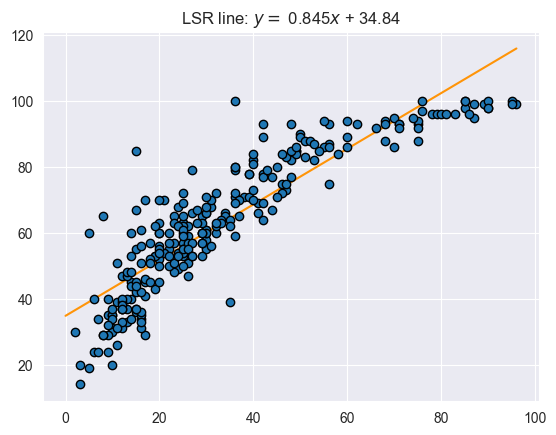
\includegraphics[height=0.35\textheight]{../../Images/CollegeTop25ontoTop10_deg1.png}
\end{center}

\end{frame}

%%%%
\begin{frame}
    \frametitle{Example}
    Here is the data set with a least squares line. The value of $R^2$ is 0.791. 
\begin{center}
    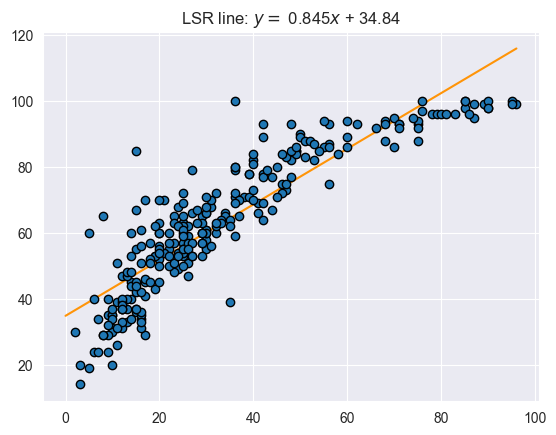
\includegraphics[height=0.35\textheight]{../../Images/CollegeTop25ontoTop10_deg1.png}
\end{center}

    \pause 
    Next, the data set with a least squares quadratic polynomial fit. The $R^2$ value is 0.854.

\begin{center}
    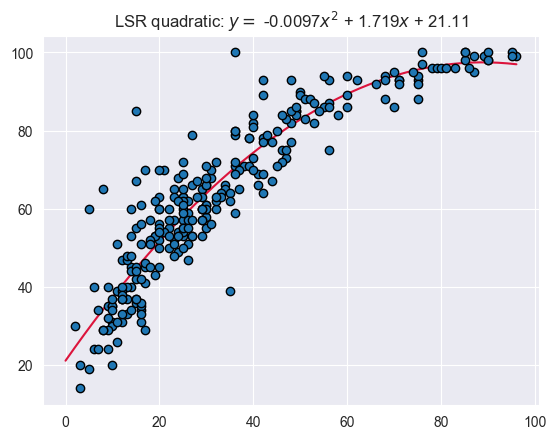
\includegraphics[height=0.35\textheight]{../../Images/CollegeTop25ontoTop10_deg2.png}
\end{center}
\end{frame}

%%%%
\begin{frame}
    \frametitle{Value of $R^2$ as polynomial degree increases}
    What will happen to the value of $R^2$ if we increase the degree of the polynomial that we fit to the data?

    \pause
    \begin{itemize}
        \item Note: Suppose that $n>d$. A Vandermonde matrix for $x$-values $x_1,x_2,\ldots, x_n$, which has $d+1$ columns (so, highest power is $x_i^d$), will have rank $d+1$ if and only if there are $d+1$ of the $x_i$ that are distinct.
        \pause
        \begin{itemize}
            \item[] \textit{If $x_1,x_2,\ldots,x_{d+1}$ are pairwise distinct, say, then the determinant of the $(d+1)\times(d+1)$ submatrix for their corresponding rows is}
            {\footnotesize
            \[{\displaystyle\prod_{1\le i<j\le d+1}(x_j - x_i)}.\]
            }
        \end{itemize}
    \end{itemize}

    \pause
    set $A_0$: the Vandermonde matrix used to fit polynomial of degree $d$; set $A_1$: the one used for polynomial of degree $d+1$. \footnote{So, $A_{1}$ has all the columns of $A_0$, and one additional column.} 
    
    From Note, as long as enough of the $x_i$ are distinct, $\operatorname{rank}(A_1) = \operatorname{rank}(A_0)+1$.

    \pause
    Meaning: $\textsf{Col}(A_0)$ is proper subspace of $\textsf{Col}(A_1)$. So, using $A_1$ makes $|y - \hat{y}|^2$ smaller. Since $\sum(y - \bar{y})^2$ is unchanged, makes $R^2$ closer to 1.
\end{frame}

\end{document}